%----------------------------------------------------------------------------
\chapter{Rendszerspecifikáció} \label{fejezet3}
%----------------------------------------------------------------------------

\section {Rendszerkövetelmények}

A rendszer specifikációit négy nagy részre oszthatjuk fel, amelyek közé tartoznak a felhasználói felület-, a jegyvásárlás-, a felhasználók- és a biztonság specifikációja. Elsőként a felhasználói felület biztosítja a felhasználó és a rendszer közötti kommunikációt. A jegyvásárlás a rendszer központi funkcionalitása, ezáltal a legkomplexebb is. Az alkalmazás lehetővé teszi a több típusú felhasználók hozzáférését a különböző funkcionalitásokhoz. Végül de nem utolsó sorban a rendszer a bizalmas adatok biztonságát is hivatott megfelelően kezelni. A specifikációk prezentálására a Visual Paradigm Online felület segítségével hoztam létre a szükséges diagramokat \cite{VPO}. A rendszer működését vizsgálni tudjuk a funkcionális- és nem funkcionális követelmény alapján.

\subsection {Funkcionális követelmények} \label{rendszerFunkcionális}

A funkcionális követelmények a rendszer funkcionalitásaira vonatkoznak, azaz meghatározzák, hogy milyen feladatokat és műveleteket kell elvégeznie a rendszernek, milyen funkciókat kell biztosítania a felhasználók számára.

\begin{itemize}
  	\item[\textbf{a,}] \textbf{Felhasználói szerepkörök:}

Az oldal böngészésének tekintetében érdemes különböző jogosultságokkal rendelkező szerepköröket kialakítani. Erre azért van szükség, mivel a rendszer több típusú felhasználó által látogatható. Ezek közül a legelső és egyben a legkevesebb funkcionalitással rendelkező az \textbf{Anonymous}, amelyek \textit{be nem jelentkezett} felhasználók, esetében ilyen funkcionális követelmények például a jegyek közötti böngészés lehetősége, a jegyek részleteinek megtekintése, valamint az email-küldés a \textit{Support} számára. Ez a funkcionalitás egy továbbfejlesztési lehetőség, mivel érdemes ennek módját egy szélesebb skálán vizsgálni. Emellett fontos, hogy az Anonymous felhasználók be tudjanak jelentkezni az oldalra vagy új felhasználói fiókot tudjanak létrehozni, és ez a bejelentkezési folyamat lehetőséget biztosít az oldalon regisztrált fiókok vagy akár más közösségi fiókok használatára is (\ref{abra:useCaseNA}).

\begin{figure}[!h]
	\centering
	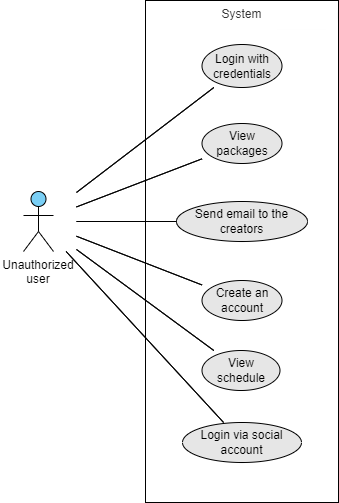
\includegraphics[scale=0.7]{images/useCaseNA}
	\caption{Use case diagram - Nem bejelentkezett felhasználó}
	\label{abra:useCaseNA}
\end{figure}
\pagebreak

A \textbf{Regular} felhasználók esetében elvárt, hogy \textit{be legyenek jelentkezve} a rendszerbe. Lehetőségük van jegyek kosárba helyezésére, megtekinteni a profiljukat, ahol lehetőségük van felhasználói név és profil kép változtatására, valamint a vásárlási előzményeiket. Az előzmények részleteinél a felhasználóknak lehetőségük van az adott jegy PIN kódjának megváltoztatására, amennyiben szükséges. A vásárlási folyamat során a felhasználók a rendelési oldalra (\textit{Checkout}) jutnak el, ahol lehetőségük van a kosárban levő jegyek mennyiségének módosítására vagy azok törlésére. Itt történik meg a fizetés és a rendelés leadása (\ref{abra:useCaseA}).

\begin{figure}[!h]
	\centering
	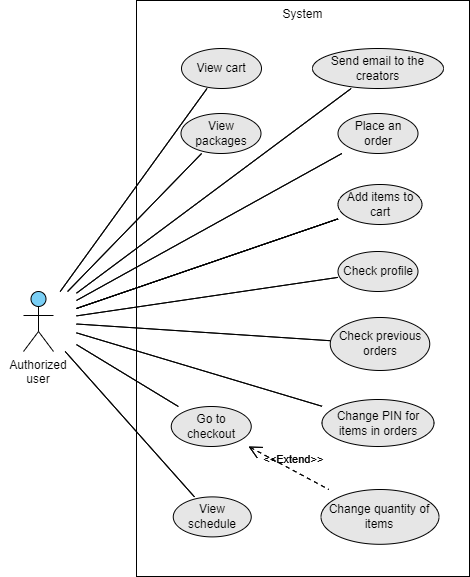
\includegraphics[scale=0.7]{images/useCaseA}
	\caption{Use case diagram - Bejelentkezett felhasználó}
	\label{abra:useCaseA}
\end{figure}
\pagebreak

Az adminisztrátorok a harmadik kategóriát alkotják a rendszerben, és különleges jogosultságokkal rendelkeznek. Az \textbf{Admin} felhasználóknak joguk van az összes korábban említett funkcionalitáshoz, mint például a jegyek kosárba helyezése, visszajelzések írása és értékelése, valamint a profiljuk kezelése és vásárlási előzményeik megtekintése. Azonban az Admin felhasználóknak további feladatuk is van, nevezetesen a jegyek hitelesítése.

Az Admin felhasználóknak lehetőségük van a jegyek hitelesítésére, amelyhez a QR kódot be kell olvasniuk vagy az adatokat manuálisan megadniuk és meg kell adniuk a PIN kódot. Ez a folyamat biztosítja, hogy csak érvényes jegyek kerüljenek elfogadásra és használatra a rendszerben. Ez a szerepkör manuálisan adható hozzá a rendszerhez, és szükség esetén módosítható.

Fontos megjegyezni, hogy bár az adminisztrátoroknak lehetőségük van jegyek vásárlására, azt kizárólag a rendszer tesztelésére és karbantartására szolgáló célokra használható. Az adminisztrátorok elsődleges felelőssége a rendszer megfelelő működésének biztosítása és a jegyek hitelesítése (\ref{abra:useCaseAdmin}).

\begin{figure}[!h]
	\centering
	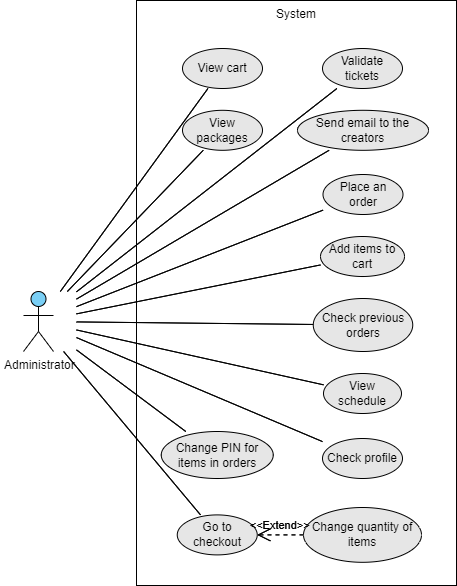
\includegraphics[scale=0.7]{images/useCaseAdmin}
	\caption{Use case diagram - Adminisztrátor}
	\label{abra:useCaseAdmin}
\end{figure}
\pagebreak

  	\item[\textbf{b,}] \textbf{Jegyvásárlás:}

A \textbf{jegyvásárlás} során a felhasználóknak számos funkcionalitást kell biztosítani. Először is, lehetőséget kell adni nekik, hogy kiválaszthassák a jegyeket és azokat kosárba helyezhessék. Emellett fontos, hogy a felhasználók módosíthassák a jegyek mennyiségét vagy akár törölhessék azokat, ha szükséges. A böngészés során pedig lehetővé kell tenni számukra, hogy részletes információkat kapjanak a jegyekről, mint például a helyszín, az időpont vagy az ár. Ez segíti őket a megfelelő döntéshozatalban és a kívánt jegyek megtalálásában.


  	\item[\textbf{c,}] \textbf{Bejelentkezés és regisztráció:}

A \textbf{bejelentkezés} és \textbf{regisztráció} lehetővé teszik a felhasználók számára, hogy saját profiljuk legyen a rendszerben, amellyel vásárlásokat tudnak végrehajtani és nyomon tudják követni azokat.

A \textbf{bejelentkezés} folyamata magában foglalja a felhasználónév és jelszó megadását vagy egy szociális fiók segítségével. A felhasználóknak lehetőségük van megadni a regisztrált felhasználónevüket és a hozzájuk tartozó jelszavukat a bejelentkezéshez. A felhasználói felületnek tartalmaznia kell egy bejelentkezés gombot, amelyre kattintva a felhasználó bejelentkezik a rendszerbe. Ezután a rendszer ellenőrzi az adatok helyességét és hitelesíti a felhasználót, hogy hozzáférjen a felhasználói funkciókhoz.

A \textbf{regisztráció} lehetőséget ad a felhasználóknak arra, hogy új fiókot hozzanak létre a rendszerben. Ehhez a felhasználóknak ki kell töltetniük egy regisztrációs űrlapot, amely tartalmazza az szükséges adatokat, például felhasználónevüket, jelszavukat, email címüket. A felületnek tartalmaznia kell egy regisztrációs gombot, amelyre kattintva a rendszer regisztrálja a felhasználót és létrehozza az új fiókját.
\end{itemize}

\subsection {Nem funkcionális követelmények}

A nem funkcionális követelmények olyan aspektusokra fókuszálnak, amelyek nem közvetlenül a rendszer funkcionalitásához kapcsolódnak, hanem inkább annak működési jellemzőit, tulajdonságait vagy környezeti tényezőit érintik.

\begin{itemize}
  	\item[\textbf{a,}] \textbf{Felhasználói szerepkörök:}

A \textbf{felhasználói szerepkörök} között egyértelmű határvonal kell legyen, hogy melyeknek mihez van jogosultságuk. A felhasználóknak könnyen és zökkenőmentesen kell tudniuk használni az oldalt függetlenül a szerepkörüktől. Fontos továbbá, hogy az egyes szerepkörökhöz tartozó jogosultságok és hozzáférési szintek megbízhatóak és biztonságosak legyenek, hogy a felhasználók csak azokhoz az információkhoz és funkciókhoz férjenek hozzá, amelyek az adott szerepkörhöz kötött.

 	 \item[\textbf{b,}] \textbf{Jegyvásárlás:}

A \textbf{jegyvásárlási} folyamatnak gyorsnak és hatékonynak kell lennie. A rendszernek képesnek kell lennie a nagyobb mennyiségű jegykezelésre és skálázhatónak kell lennie, hogy a jegyvásárlás során ne jelentkezzenek teljesítménybeli problémák. Emellett a jegyvásárlás folyamatának biztonságosnak is kell lennie, és megfelelő védelmi intézkedéseket kell tartalmaznia az adatbiztonság érdekében. Ilyen intézkedések például a titkosított adatátvitel vagy a vásárlói adatok megfelelő védelme.

	 \item[\textbf{c,}] \textbf{Bejelentkezés és regisztráció:}

A \textbf{bejelentkezés és regisztráció} folyamata kapcsán a nem funkcionális követelmények között szerepel, hogy a folyamatnak biztonságosnak kell lennie. A bejelentkezési és regisztrációs folyamatnak megfelelő hitelesítési és azonosítási mechanizmusokat kell tartalmaznia. Emellett a folyamatnak gyorsnak és felhasználóbarátnak kell lennie, hogy a felhasználók könnyedén és zökkenőmentesen tudjanak bejelentkezni vagy regisztrálni. A felhasználóknak egyszerű és intuitív felhasználói felületet kell biztosítani a bejelentkezéshez és regisztrációhoz, hogy könnyen megadhassák szükséges információikat és végrehajthassák az adott folyamatot.
\end{itemize}


\section {Felhasználói követelmények}

\begin{itemize}
  	\item[\textbf{a,}] \textbf{Funkcionalitások:}

A főbb funkcionalitások tervezésénél, amelyekről szó volt a funkcionális rendszer követelmények alfejezet (\ref{rendszerFunkcionális}) keretében, figyelembe vettem, hogy azok a lehető legjobban betöltség a feladatukat, így a felhasználók zökkenőmentesen tudják használni a rendszert. Figyelembe vettem az implementáció során a funkcionalitások teljesítményének, megbízhatóságának és használhatóságának a fontosságát.

	\item[\textbf{b,}] \textbf{Felhasználói felület:}

A rendszer felhasználói felületének fejlesztése első sorban arra irányult, hogy intuitív és könnyen érthető legyen, ezáltal a felhasználók ne tapasztaljanak nehézségeket vagy zavarokat az alkalmazás használata során. Egy felhasználó első benyomása határozza meg a legnagyobb mértékben a rendszerről alkotott véleményét, ezért kellő figyelmet fordítottam arra, hogy az oldal letisztult legyen, elkerülve a félrevezető utasításokat és funkcionalitásokat. A felhasználó az oldal első látogatásakor értesül az oldal céljáról egy felugró ablakban.

	\item[\textbf{c,}] \textbf{Teljesítmény és megbízhatóság:}

Az alkalmazás teljesítménye több komponensből áll össze, amelyek közé tartoznak a reakcióidő, válaszkészség, stabilitás és rendelkezésre állás. Fontosnak tartottam, hogy az alkalmazás gyorsan és megbízhatóan működjön, hogy a felhasználók ne érezzenek frusztráló lassulásokat vagy hibákat. Persze a hibák teljes mértékű elkerülése majdnem lehetetlen a szoftver rendszerek esetében, mivel az emberi hiba lehetősége mindig jelen van. Arra törekedtem, hogy minimalizálva legyen a hibák előfordulásának lehetősége és megelőző intézkedéseket vezettem be. Ide tartoznak azok a megfelelő hibaüzenetek is, amelyek kisebb vagy nagyobb hibák esetén is célravezető módon informálják a felhasználót, hogy ez a hiba miként befolyásolja a rendszer további működését vagy adott esetben mit tud tenni a felhasználó a hiba elkerülése ellen.

	\item[\textbf{d,}] \textbf{Profilkezelés:}

A felhasználók számára fontos szempont, hogy hozzáférjenek a saját adataikhoz egy oldalon és módosítani tudják őket. Erre a célra hoztam létre egy aloldalt, ahol kényelmesen lehet profil képet, felhasználónevet módosítani és a rendelési előzmenyeket visszanézni. Továbbá lehetőségük van, hogy az egyes rendelésekhez új PIN kódot rendeljenek.

	\pagebreak
	\item[\textbf{e,}] \textbf{Kompatibilitás:}

Az alkalmazás elsősorban a asztali számítógépekre lett optimalizálva, viszont egy következő továbbfejlesztési lehetőség lenne, hogy reszponzív legyen, ezáltal mobilon és táblagépen is könnyedén kezelhető legyen az oldal. A rendszer kompatibilis a közismert modern böngészők mindegyikével, mint a Microsoft Edge, Google Chrome, Mozilla Firefox, Apple Safari vagy az Opera (\ref{abra:browserLogos}).

\begin{figure}[!h]
	\centering
	
\includegraphics[scale=0.2]{images/browserLogos}
	\caption{Web böngészők}
	\label{abra:browserLogos}
\end{figure}
\end{itemize}